\section{The triangular chart and monomial sections}\label{tri:section}

We now identify the evaluated monomial symmetric polynomials with single
positive sections.  The auxiliary graph used for this purpose contains every
naturally labeled unit interval graph as an ordered induced subgraph.
All lattice vectors in this section belong to the free lattice on the
vertices; the extra dual directions, if used to make the skew form
nondegenerate, never occur in their support.

Positive theta sections do not yet give elementary positivity: we must
identify each evaluated monomial symmetric function with a single such
section.  We first introduce an auxiliary graph with a distinguished
independent set of vertices.  Repeated rotations constrain the incoming
coefficients, but those constraints alone do not force the desired
identity.  A separate analysis of the degree-one symmetric function
will give a positive support bound for its higher-degree analogues;
that bound is what makes the final subtraction argument possible.

\subsection{The chart and its rotations}

Fix an integer $D\geq 1$, and put $n_0=D-1$.  There are anchors
$d_1,\ldots,d_D$ at the integer times $1,\ldots,D$.  For each
$1\leq j\leq i\leq n_0$ there is a bridge $b_{j,i}$ at time
$i+\theta_{j,i}$, where $0<\theta_{j,i}<1$.  The phases are distinct.
For $D>1$, their increasing order is
\begin{equation}\label{tri:phase-order}
 (n_0,n_0);\quad (n_0-1,n_0-1),(n_0-1,n_0);\quad\ldots;\quad
 (1,1),(1,2),\ldots,(1,n_0).
\end{equation}
The index $i$ is the \emph{level}, and $j$ is the \emph{row}.
Two vertices are adjacent precisely when their times differ by less than
$1$.  In particular, the anchors are independent, bridges on one level
form a clique, and bridges on neighboring levels are adjacent precisely
when the bridge on the higher level has the earlier phase.

Use the vertex names also for their independent lattice vectors.  The
skew form has $\Omega(b,a)=1$ when $a$ precedes $b$ and they are adjacent,
and is zero on nonedges.  We use the quantum torus normalization
$X_aX_b=v^{\Omega(a,b)}X_{a+b}$.
The independent-set elements
\[
 E_k=e_k(Y)=\sum_{\substack{I\text{ independent}\\ |I|=k}}
 X_{\sum_{a\in I}a},\qquad U=E_1,
\]
commute by Proposition~\ref{graph:commutation}.  An independent set has at
most $D$ vertices: its ordered times have successive differences at least
$1$ and lie in $[1,D]$.  Thus $P(Y)$ is defined for every symmetric
polynomial $P$ in $D$ variables.

\begin{lemma}[Embedding]\label{tri:embedding}
Every naturally labeled unit interval graph on $n$ vertices occurs as
an ordered induced subgraph on $n$ selected bridges of a triangular
chart.  The times and phases may all be chosen rationally.
\end{lemma}

\begin{proof}
For $n=0$ take $D=1$.  For $n>0$, first construct strictly increasing
positive rational times
$t_1,\ldots,t_n$, with distinct nonzero fractional parts, such that
$a<b$ is an edge exactly when $t_b-t_a<1$.
Choose any positive nonintegral rational $t_1$.  For $k\geq2$, suppose
the times through $t_{k-1}$ have been chosen.  The earlier
neighbors of $k$ form a suffix $s,s+1,\ldots,k-1$ because the defining
function $h$ is weakly increasing.  If that suffix is empty, choose
$t_k>t_{k-1}+1$.  Otherwise choose
\[
 \max\{t_{k-1},t_{s-1}+1\}<t_k<t_s+1,
\]
omitting $t_{s-1}+1$ when $s=1$.
The interval is nonempty: when $s>1$ we have $t_{s-1}<t_s$, and either $s=k-1$ or
$s$ and $k-1$ are already adjacent, since $h(s)\geq k$.
These inequalities give exactly the required earlier neighbors.
At each step an open interval of choices remains, so rational choices
avoiding all previously used fractional parts are possible.

Shift every time by a common integer so that every level
$\lfloor t_a\rfloor$ is at least $n$, and then choose $D$ so large that
all these levels are at most $D-1$.  Order the $n$ selected vertices by
increasing fractional part and assign them, in that order, to the rows
$n,n-1,\ldots,1$.  A vertex of level $i\geq n$ has an available bridge
in every one of these rows.  Set that bridge's phase equal to the
vertex's fractional part.  There is one prescribed phase per selected
row, and they increase in the order~\eqref{tri:phase-order}.
Insert all the other phases as rational numbers between these prescribed
values, respecting the same order.  The selected bridges have exactly
the shifted original times, so their ordered induced graph is the
given graph.
\end{proof}

Give every vertex weight $1$.  On each level take the successive
forward differences in the list
\begin{equation}\label{tri:level-list}
 d_i,b_{i,i},b_{i-1,i},\ldots,b_{1,i},d_{i+1}.
\end{equation}
Let $C$ be the union of these roots.  Concatenating these lists gives
one ordered list of all vertices, and its successive differences,
together with $d_1$, form a lattice basis.  In particular $C$ is a
basis of the weight-zero lattice and
$C^+=\sum_{c\in C}\N c$ is a free pointed cone.
Every simple root carries the unit $D_c$ of
Lemma~\ref{wall:unit}.
For any vertex $a$, the difference $a-d_1$ lies in $C^+$; consequently
every homogeneous evaluation $P(Y)$ of degree $N$ has support in
\begin{equation}\label{tri:support-cone}
 Nd_1+C^+.
\end{equation}
Here and below $P(Y)$ also denotes the section whose value in the
all-negative chamber is this polynomial.

A \emph{rotation} moves the globally first bridge $b$, on level $i$,
to the last phase and replaces its vector by
\begin{equation}\label{tri:rotation}
 b'=b+\delta_i,\qquad \delta_i=d_{i+1}-d_i,
 \qquad p=b-d_i.
\end{equation}
The anchors are fixed.  At this step
\[
 \Omega(p,d_i)=1,\quad \Omega(p,d_{i+1})=-1,\quad
 \Omega(p,b)=1,
\]
and $p$ pairs to zero with every other vertex.  Thus the root mutation
$p\mapsto-p$, $c\mapsto c+[-\Omega(p,c)]_+p$ of
Theorem~\ref{wall:mutation} gives precisely the new forward lists.
On the moved level, the next and the last old gaps each receive $p$;
when these are the same gap it receives $2p$.  The root $-p$ is the
new final gap $d_{i+1}-b'$.  All other gaps are unchanged.
Pairing the new vertex vectors also gives the interval-graph rule with
$b'$ last in phase order.

\begin{lemma}[Polynomial comparison under rotation]\label{tri:rotation-comparison}
Let $Y'$ be the alphabet after one rotation.  For every symmetric
polynomial $P$,
\begin{equation}\label{tri:polynomial-comparison}
 P(Y)=\Ad(D_p)P(Y').
\end{equation}
Both sides are finite Laurent polynomials, so the actual incoming
coefficients satisfy
\begin{equation}\label{tri:incoming-rotation}
 A_m(P(Y))=A_{m+[-\Omega(p,m)]_+p}(P(Y')).
\end{equation}
\end{lemma}

\begin{proof}
It suffices to prove~\eqref{tri:polynomial-comparison} for $E_k$.
Relative to all vertices outside $\{d_i,b,d_{i+1}\}$, the old bridge
$b$ has the same neighbors as $d_i$, whereas the new bridge $b'$ has
the same neighbors as $d_{i+1}$.  The elementary conjugation formulas
give
\begin{align*}
 \Ad(D_p)X_{d_i}&=X_{d_i}+X_b,\\
 \Ad(D_p)(X_{d_{i+1}}+X_{b'})&=X_{d_{i+1}},\\
 \Ad(D_p)X_{d_i+d_{i+1}}&=X_{d_i+d_{i+1}}.
\end{align*}
For completeness, the first identity is the centered binomial formula
with pairing $1$ and $d_i+p=b$; the second is its inverse with pairing
$-1$ and $d_{i+1}+p=b'$; the last uses pairing zero.
Fix an independent set outside this triple.  Its monomial commutes with
$X_p$.  The displayed identities match all ways to extend it by no
vertex, one vertex, or the independent pair $\{d_i,d_{i+1}\}$.
Their sum proves the assertion for each $E_k$.
Since conjugation is an algebra automorphism and the $E_k$ commute, the
assertion follows for $P$.  Theorem~\ref{wall:mutation}, applied to these
finite polynomial values, now gives~\eqref{tri:incoming-rotation}.
\end{proof}

Repeat the rotations indefinitely.  One \emph{period} moves every
bridge once.  After $L$ periods the bridge originally on level $i$ is
$b+L\delta_i$, the phase order is again~\eqref{tri:phase-order}, and
the roots are denoted by $C_L$.

\subsection{Stationarity and pure incoming coefficients}

\begin{lemma}[Stationary incoming labels]\label{tri:stationary}
Let $P$ be a homogeneous symmetric polynomial of degree $N$, and
suppose $A_m(P(Y))\ne0$.
Write the label in the original vertex basis as
\[
 m=\sum_{i=1}^D\nu_i d_i+\sum_{j\leq i}\kappa_{j,i}b_{j,i},
 \qquad K_i=\sum_{j=1}^i\kappa_{j,i},\qquad K_0=K_D=0.
\]
Then
\begin{equation}\label{tri:stationary-conditions}
 K_i=0\quad(1\leq i<D),\qquad
 \xi_{j,i}:=\Omega(b_{j,i}-d_i,m)\geq0\quad(1\leq j\leq i<D).
\end{equation}
The lattice label $m$ is fixed by every tropical step in
Equation~\eqref{tri:incoming-rotation}.
If $m$ is pure, meaning that all its bridge coordinates vanish, then
$m=\sum_i\mu_i d_i$, where
$\mu_1\geq\cdots\geq\mu_D\geq0$ and $\sum_i\mu_i=N$.
\end{lemma}

\begin{proof}
For $D=1$ the support bound already gives $m=Nd_1$, so assume $D>1$.
Track the nonzero coefficient using~\eqref{tri:incoming-rotation}.
At each stage use the current vertex basis to write its current label
as $\sum\nu_i d_i+\sum\kappa_b b$.
When $b$ on level $i$ is moved, put
$t=[-\Omega(b-d_i,m)]_+$.  Reexpressing
$m+t(b-d_i)$ using $b'=b+d_{i+1}-d_i$ gives
\begin{equation}\label{tri:coordinate-step}
 \kappa_b'=\kappa_b+t,\qquad
 \nu_i'=\nu_i+\kappa_b,\qquad
 \nu_{i+1}'=\nu_{i+1}-\kappa_b',
\end{equation}
with all other coordinates unchanged.
Thus every individual bridge coordinate, and every $K_i$, is a
nondecreasing integer along the tracked sequence.

In every chart the current polynomial has support
$Nd_1+C^+$.  Triangularity of incoming coordinates preserves this
lower support bound.  In particular the cut just before $d_{i+1}$
gives the nonnegative deficit
\begin{equation}\label{tri:cut-deficit}
 B_i=N-\sum_{j\leq i}(\nu_j+K_j)\geq0.
\end{equation}
Equation~\eqref{tri:coordinate-step} shows that $B_i$ changes only at
moves on level $i$, and then changes by $-\kappa_b'$.
If $K_i$ were positive at any stage, each subsequent complete period
would decrease $B_i$ by at least this positive integer: each bridge's
coordinate at its next move is at least its coordinate at the start
of the period.  This contradicts~\eqref{tri:cut-deficit}.  Therefore
$K_i\leq0$ at every stage.

Since each $\kappa_b$ is nondecreasing and their level sum is bounded
above by zero, each $\kappa_b$ is bounded above as well; one may use
the initial lower bounds for the other bridge coordinates on its
level.  All these integer sequences stabilize.  From that time on
every $t$ is zero, and the \emph{lattice vector} of the tracked label
is a fixed vector $m_*$.  Its anchor coordinates in the moving
vertex basis need not be fixed.

At the event originally named $b$ on level $i$, the root in period
$L$ is $b-d_i+L\delta_i$.  For all sufficiently large $L$ its pairing
with $m_*$ is nonnegative.  Its slope as a function of $L$ is
\begin{equation}\label{tri:concavity}
 \Omega(\delta_i,m_*)=2K_i-K_{i-1}-K_{i+1}\geq0.
\end{equation}
Indeed $\delta_i$ pairs by $2$ with a bridge on level $i$, by $-1$
with a bridge on either neighboring level, and by zero with all
other vertices.  The sequence $K_0,\ldots,K_D$ is therefore discretely
concave.  With zero endpoints it lies above the zero chord, so
$K_i\geq0$.  Together with $K_i\leq0$, this proves $K_i=0$.

The slopes in~\eqref{tri:concavity} now vanish.  Consequently $m_*$
pairs with every original event root just as it does with its late
counterparts; all these pairings are nonnegative.  It is fixed by
every tropical step, including the earlier ones.  Each map
$T_p(x)=x+[-\Omega(p,x)]_+p$ is invertible, with inverse
$x\mapsto x-[-\Omega(p,x)]_+p$, because adding $p$ leaves its pairing
with $p$ unchanged.  Applying these inverses recovers the same $m_*$
at every earlier stage.  This proves~\eqref{tri:stationary-conditions}
for the original label.

For a pure label, $\xi_{j,i}=\mu_i-\mu_{i+1}$, so its coordinates
decrease.  The last cut in~\eqref{tri:cut-deficit} says $\mu_D\geq0$.
Weight is unchanged by every operation, hence $\sum_i\mu_i=N$.
\end{proof}

\begin{example}\label{tri:mixed-stationary}
Stationarity permits mixed labels.  For $D=3$ the phase order is
$b_{2,2},b_{1,1},b_{1,2}$, and
\[
 m=d_2+b_{1,2}-b_{2,2}
\]
satisfies $K_1=K_2=0$ and
$\xi_{1,1}=\xi_{2,2}=\xi_{1,2}=0$.  Moreover,
\[
 m-d_1=(b_{1,1}-d_1)+(d_2-b_{1,1})+(b_{1,2}-b_{2,2})\in C^+.
\]
It is therefore a stationary candidate of weight $1$, although its
$b_{2,2}$ coordinate is negative.  Its incoming coefficient in $U$
will be excluded by a separate argument.
\end{example}

\begin{lemma}[Pure coefficient extraction]\label{tri:pure}
Let $P$ be a homogeneous symmetric polynomial of degree $N$, and let
$m=\sum_i\mu_i d_i$ with
$\mu_1\geq\cdots\geq\mu_D\geq0$ and $\sum_i\mu_i=N$.
For commuting indeterminates $z_1,\ldots,z_D$,
\begin{equation}\label{tri:pure-formula}
 A_m(P(Y))=[z_1^{\mu_1}\cdots z_D^{\mu_D}]P(z_1,\ldots,z_D).
\end{equation}
\end{lemma}

\begin{proof}
We choose a single sufficiently large integer $L$ after fixing the
finite set of possible increments for this coefficient.
Since $m-Nd_1\in C^+$, that set is
\begin{equation}\label{tri:finite-candidates}
 \mathcal R_m=\{r\in C^+:0<r\leq m-Nd_1\},
\end{equation}
where $r\leq s$ means $s-r\in C^+$.  It is finite because $C$ is a
finite free basis.  Its members have bounded original vertex
coordinates, independently of $L$.

Define a covector by
\begin{equation}\label{tri:test-covector}
 Q_L(d_i)=D-i,\qquad Q_L(b-d_i)=L-\theta_b
 \quad\text{for an original bridge on level }i.
\end{equation}
For the moved bridge $b^{(L)}=b+L\delta_i$ its value is
$Q_L(b^{(L)})=D-i-\theta_b$.  The values strictly decrease along
each moved forward list, so $Q_L$ is in the all-negative chamber
for $C_L$.
Every mutation cut used in the first $L$ periods has root
$p_b^{(\ell)}=b-d_i+\ell\delta_i$ for some $0\leq\ell<L$, and
\[
 Q_L(p_b^{(\ell)})=L-\theta_b-\ell>0,
 \qquad \Omega(p_b^{(\ell)},m)=\mu_i-\mu_{i+1}\geq0.
\]
Hence the entire ray $Q_L+sV(m)$, $s\geq0$, lies on the identity
side of all these cuts.  Repeated application of
Theorem~\ref{wall:mutation} identifies the wall systems there by
the identity on lattice vectors, and identifies the section at
$Q_L$ with the finite graph polynomial in the chart after $L$
periods.

Consider a wall capable of changing the coefficient of $X_m$ along
this ray.  Any positive increment on its ray belongs to
$\mathcal R_m$: the starting exponent is at least $Nd_1$ in the
original cone.  Furthermore an actual contributing wall root belongs
to $C_L^+$, by the successive identity-side wall identifications.
This assertion concerns the roots on those walls; it does not assert
an inclusion between the entire old and new cones.

For $r\in\mathcal R_m$, write its original coordinates as
$\nu_i(r),\kappa_b(r)$ and put
\[
 P_i(r)=\sum_{j\leq i}(\nu_j(r)+K_j(r)).
\]
As a \emph{fixed vector} reexpressed after $L$ periods, $r$ has
unchanged bridge coordinates and anchor coordinates
\begin{equation}\label{tri:moving-prefix}
 \nu_i^{(L)}(r)=\nu_i(r)+L\bigl(K_i(r)-K_{i-1}(r)\bigr).
\end{equation}
Thus its moved prefix is $P_i(r)+LK_i(r)$.  A weight-zero member of
$C_L^+$ has nonpositive prefixes, giving
$P_i(r)+LK_i(r)\leq0$.
Choose $L$ larger than all $-P_i(r)$ for $r\in\mathcal R_m$ and
$1\leq i<D$.  Since the $K_i(r)$ are integers, every contributing
candidate must then satisfy $K_i(r)\leq0$ for all $i$.

There is also an $L$-independent quantity $q_0(r)$ such that
\[
 Q_L(r)=L\sum_iK_i(r)+q_0(r).
\]
Increasing the same $L$ to exceed all $q_0(r)$ makes $Q_L(r)<0$
whenever some $K_i(r)<0$ and all are nonpositive.  For every
contributing candidate,
\begin{equation}\label{tri:no-crossing-pairing}
 \Omega(r,m)=\sum_{i=1}^{D-1}K_i(r)(\mu_i-\mu_{i+1})\leq0.
\end{equation}
If some $K_i(r)<0$, then
$(Q_L+sV(m))(r)=Q_L(r)+s\Omega(r,m)<0$ for every $s\geq0$,
so the ray never crosses its hyperplane.  If all $K_i(r)$ vanish,
the pairing is zero.  A wall on this ray fixes every monomial
$X_{m-ar}$, since $\Omega(r,m-ar)=0$, and cannot change the
$X_m$ coefficient.

All these comparisons require only finitely many orders for the
fixed target and the chosen $L$.  Perturb $Q_L$ by a sufficiently
small generic covector at these orders, retaining the strict cut
inequalities and the strict negative inequalities just established.
This also handles any walls parallel to the unperturbed ray; their
zero-pairing actions still fix the target coefficient.  For large
$s$, the target coefficient at $Q_L+sV(m)$ is the incoming
coefficient by its definition.  It therefore equals the coefficient
at $Q_L$.

Finally, in the moved vertex basis the target $m$ still has zero
bridge coordinates.  Every graph monomial using a bridge has a
positive coordinate at that bridge, and hence cannot contribute.
Suppressing all bridges leaves the independent anchors; their
monomials commute without powers of $v$.  The coefficient at $Q_L$
is exactly the right side of~\eqref{tri:pure-formula}.
\end{proof}

\subsection{The linear section and its gap recurrence}

\begin{lemma}\label{tri:linear}
In the all-negative chamber of the triangular chart,
\[
 U=\Theta_{d_1}.
\]
\end{lemma}

\begin{proof}
Assume $D>1$, as the assertion for $D=1$ is immediate.  Take any
label $m$ with $A_m(U)\ne0$.  By the support bound and
Lemma~\ref{tri:stationary}, the vector $m-d_1$ is a nonnegative
integer combination of the forward gaps, its bridge totals $K_i$
vanish, and all $\xi_{j,i}$ are nonnegative.

On level $i$, let $u_{j,i}$ be the coefficient of the gap immediately
following $b_{j,i}$ in~\eqref{tri:level-list}.  Put $a_i=u_{1,i}$,
and $a_0=0$.  The sum of the bridge coordinates on that level is
the first gap coefficient minus the last gap coefficient.  Thus
$K_i=0$ says that the initial gap $b_{i,i}-d_i$ also has coefficient
$a_i$.  In particular both end gaps are included in this notation.
Figure~\ref{tri:gap-figure} illustrates these coefficients.
All the $u_{j,i}$ and $a_i$ are nonnegative integers.

\begin{figure}[ht]
\centering
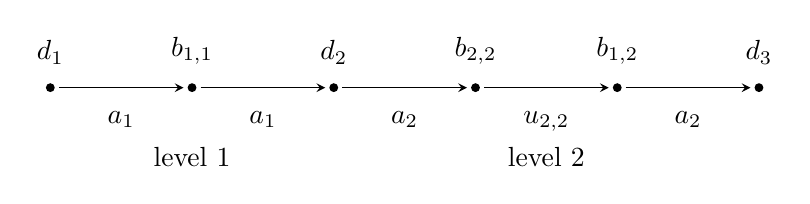
\begin{tikzpicture}[x=0.9cm,y=0.8cm,>=stealth]
 \foreach \x/\name in {0/d_1,2/b_{1,1},4/d_2,6/b_{2,2},8/b_{1,2},10/d_3}
   {\fill (\x,0) circle (1.6pt);\node[above=5pt] at (\x,0) {$\name$};}
 \draw[->] (0.12,0)--node[below=5pt] {$a_1$}(1.88,0);
 \draw[->] (2.12,0)--node[below=5pt] {$a_1$}(3.88,0);
 \draw[->] (4.12,0)--node[below=5pt] {$a_2$}(5.88,0);
 \draw[->] (6.12,0)--node[below=5pt] {$u_{2,2}$}(7.88,0);
 \draw[->] (8.12,0)--node[below=5pt] {$a_2$}(9.88,0);
 \node at (2,-1.1) {level $1$};
 \node at (7,-1.1) {level $2$};
\end{tikzpicture}
\caption{The gap coefficients for $D=3$.  The horizontal order is time
order, drawn schematically; phase order is
$b_{2,2},b_{1,1},b_{1,2}$.  Vanishing bridge totals equate the two
end coefficients on each level.}
\label{tri:gap-figure}
\end{figure}

We spell out the pairing calculation underlying the recurrence.
For $p=b_{j,i}-d_i$, its values on the same-level bridges are $2$
before $b_{j,i}$, $1$ at $b_{j,i}$, and $0$ after it.  On bridges
of a neighboring level its values are $-1$ before this phase and
$0$ after it.  Its anchor values are $1$ at $d_i$, $-1$ at
$d_{i+1}$, and zero elsewhere.
Evaluate these values on successive differences.
The contribution on its own level is minus the two gaps adjacent to
$b_{j,i}$: the additional contributions from the two end gaps cancel
because their coefficients agree.  On level $i-1$ the same endpoint
cancellation leaves the coefficient of the gap containing the phase
of $b_{j,i}$; on level $i+1$ that coefficient is obtained directly.
The contribution of the initial $d_1$ is $\boldsymbol1_{i=1}$.
With nonexistent terms interpreted as zero, this gives
\begin{equation}\label{tri:gap-pairing}
\begin{split}
 \xi_{j,i}={}&\boldsymbol1_{i=1}-u_{j,i}
 -\begin{cases}u_{j+1,i},&j<i,\\a_i,&j=i,\end{cases}\\
 &+\begin{cases}u_{j,i-1},&j<i,\\a_{j-1},&j=i,\end{cases}
 +u_{j+1,i+1}.
\end{split}
\end{equation}
Indeed the upper neighboring gap follows the event in row $j+1$;
the lower neighboring gap follows the event in row $j$ when $j<i$,
and is its initial gap when $j=i$.

Set
\[
 T_{j,i}=u_{j,i}-u_{j+1,i+1},\qquad 1\leq j\leq i\leq n_0,
\]
again using zero for nonexistent terms.  Equation~\eqref{tri:gap-pairing}
is equivalently
\begin{equation}\label{tri:gap-recurrence}
 \begin{aligned}
 T_{j,j}&=\boldsymbol1_{j=1}+a_{j-1}-a_j-\xi_{j,j},\\
 T_{j,i}&=T_{j,i-1}-\xi_{j,i} &&(i>j).
 \end{aligned}
\end{equation}
Each row of $T$ is weakly decreasing and ends in
$T_{j,n_0}=u_{j,n_0}\geq0$.  Hence every $T_{j,i}\geq0$.
The row-start inequalities then give $a_1\leq1$ and
$a_j\leq a_{j-1}$ for $j>1$.  Integrality shows that
\[
 a_1,\ldots,a_{n_0}=\underbrace{1,\ldots,1}_{e},0,\ldots,0
\]
for some $0\leq e\leq n_0$.
The case $e=n_0$ is impossible: every row-start upper bound in
Equation~\eqref{tri:gap-recurrence} would be zero, giving $T=0$
and then $u=0$, contrary to $a_1=1$.

All rows of $T$ except row $e+1$ have zero row-start upper bound.
Row $e+1$ has upper bound $1$, so its nonzero entries form an
initial stretch of ones in columns $e+1,\ldots,t$, for some
$e\leq t\leq n_0$; $t=e$ denotes an empty stretch.
The definition of $T$ telescopes along southeast diagonals:
\begin{equation}\label{tri:diagonal-recovery}
 u_{j,i}=\sum_{a\geq0}T_{j+a,i+a}.
\end{equation}
In particular $u_{1,i}=a_i$ is $1$ exactly for $1\leq i\leq t-e$.
Comparison with its already known run of length $e$ gives
$t=2e$.  Thus every positive gap coefficient is on a level
$i\leq2e$.  From~\eqref{tri:gap-recurrence}, a positive $\xi_{j,i}$
can occur only at the drop after this stretch, in level $2e+1$
(if that level exists).  In particular all $\xi_{j,i}$ on a
positively used level are zero.  When $e=0$, every gap coefficient is
zero and the possible positive value is the initial term $\xi_{1,1}$;
thus the same conclusion includes the empty stretch.

Every positively used forward root therefore pairs trivially with
$m$.  For an interior gap its pairing is the difference of the
two adjacent $\xi$ values; for the first gap it is $\xi_{i,i}$.
For the last gap it is
\[
 \Omega(d_{i+1}-b_{1,i},m)
   =\Omega(\delta_i,m)-\xi_{1,i}=0,
\]
since $K=0$ gives $\Omega(\delta_i,m)=0$ by
Equation~\eqref{tri:concavity}.  This verifies both end gaps as well
as the interior ones.

A wall increment capable of changing $[X_m]$ lies in the finite
interval $0<r\leq m-d_1$.  As $C$ is free, such an $r$ can use
only positively used gaps, and hence $\Omega(r,m)=0$.
Conjugation on that ray fixes every possible predecessor of $m$.
It follows that transport from the all-negative chamber to the
incoming direction does not change this coefficient, so
$A_m(U)=[X_m]U$.
The only vertex exponent consistent with
Lemma~\ref{tri:stationary} is $d_1$: bridges have nonzero level
total, and a pure unit vector is dominant only at the first anchor.
Therefore the only nonzero incoming coefficient of $U$ is
$A_{d_1}(U)=1$.  The definition of the incoming basis proves
$U=\Theta_{d_1}$.
\end{proof}

\subsection{Positive domination and the monomial identity}

\begin{lemma}[Vertex support before subtraction]\label{tri:domination}
For every partition $\mu\vdash N$ with at most $D$ parts, padded by
zeroes, put $x_\mu=\sum_i\mu_i d_i$.  In the all-negative chamber,
$\Theta_{x_\mu}$ has nonnegative vertex exponents and coefficients
in $\N[v,v^{-1}]$, and is a finite Laurent polynomial.  More
precisely, coefficientwise in both vertex exponents and $v$,
\begin{equation}\label{tri:positive-domination}
 \frac{N!}{\prod_i\mu_i!}\,\Theta_{x_\mu}\ \leq\ U^N.
\end{equation}
\end{lemma}

\begin{proof}
Lemma~\ref{tri:linear} and Corollary~\ref{wall:product} give a
nonnegative incoming expansion of $U^N$.
Lemma~\ref{tri:pure}, applied to $(z_1+\cdots+z_D)^N$, gives
\[
 A_{x_\mu}(U^N)=\frac{N!}{\prod_i\mu_i!}>0.
\]
Every section in this expansion has nonnegative coefficients in
every chamber by Theorem~\ref{wall:positivity}.  Retaining the one
displayed summand therefore gives~\eqref{tri:positive-domination}.
The right side is a finite Laurent polynomial with nonnegative
vertex exponents and nonnegative integral coefficients in $v$.
No coefficient outside that finite support, and no negative
vertex coordinate, can occur in the retained positive summand.
This proves all the claims, including finiteness of its Laurent
coefficients.  The case $N=0$ is the identity section.
\end{proof}

\begin{theorem}[Monomial sections]\label{tri:monomial}
For every partition $\lambda$ with at most $D$ parts, padded by
zeroes to length $D$, one has in the all-negative chamber
\begin{equation}\label{tri:monomial-identity}
 m_\lambda(Y)=\Theta_{\sum_{i=1}^D\lambda_i d_i}.
\end{equation}
In particular,
\begin{equation}\label{tri:elementary-identity}
 E_k=\Theta_{d_1+\cdots+d_k}\qquad(0\leq k\leq D).
\end{equation}
\end{theorem}

\begin{proof}
For $D=1$ the cone is trivial and the assertion is immediate.
Otherwise set $N=|\lambda|$ and $x_\lambda=\sum_i\lambda_i d_i$.
The polynomial $m_\lambda(Y)$ has nonnegative vertex exponents:
it is a polynomial in the independent-set generators, each of
which has this support property.  This assertion concerns its
exponent support and does not assume coefficient positivity.
Lemma~\ref{tri:domination} already gives the same support property
for $\Theta_{x_\lambda}$.

By Lemmas~\ref{tri:stationary} and~\ref{tri:pure}, the pure
incoming coefficients of $m_\lambda(Y)$ are $1$ at $x_\lambda$
and zero at every other pure label.  Indeed $m_\lambda$ is the
sum of the distinct ordinary monomials in the orbit of $\lambda$,
and that orbit contains exactly one dominant vector.
Subtract the indicated section and write
\[
 F=m_\lambda(Y)-\Theta_{x_\lambda}.
\]
Its ordinary support still has nonnegative vertex coordinates,
all its pure incoming coefficients vanish, and both its ordinary
and incoming support lie in $Nd_1+C^+$.

If an incoming coefficient remains nonzero, its label $m$ is
mixed and satisfies $K_i(m)=0$ by Lemma~\ref{tri:stationary};
subtracting $\Theta_{x_\lambda}$ changes only one pure incoming
coefficient.  A nonzero bridge-coordinate vector with zero sum
on each level has some negative bridge coordinate.
Among all remaining labels choose one with minimum height in
$Nd_1+C^+$, where the height is the sum of its nonnegative simple
root coordinates.  A minimum exists in $\N$, even if the incoming
expansion is infinite.  Incoming triangularity says that the
ordinary coefficient at this label equals its incoming
coefficient plus contributions from strictly lower incoming
labels.  There are no such nonzero lower terms by the choice of
height.  Hence $[X_m]F=A_m(F)\ne0$, contradicting the negative
bridge coordinate of $m$ and the vertex support already proved.
No coefficient remains, proving~\eqref{tri:monomial-identity}.
Finally $m_{(1^k)}=e_k$ gives~\eqref{tri:elementary-identity}.
\end{proof}


\begin{corollary}[Elementary positivity]\label{tri:positivity}
Let $G$ be a natural unit interval graph on $n$ vertices, and put
$M=|E(G)|$.  In its elementary expansion
\[
 \chi_G(X;q)=\sum_{\lambda\vdash n}c_\lambda(q)e_\lambda(X),
\]
every $c_\lambda(q)$ belongs to $\N[q]$ and has degree at most $M$.
For a triangular embedding with $D\geq n$, let $u$ be the sum of the
selected vertex exponents and set $x_\lambda=\sum_i\lambda_i d_i$,
padding $\lambda$ by zeroes.  Then
\begin{equation}\label{tri:positive-coefficient}
 [X_u]\Theta_{x_\lambda}^{H_-}
   =v^{-M}c_\lambda(v^2)
   \in\sum_{d=0}^{M}\N v^{2d-M},
\end{equation}
where $H_-$ is the all-negative chamber.
\end{corollary}

\begin{proof}
Choose the embedding of Lemma~\ref{tri:embedding}, taking $D\geq n$.
Proposition~\ref{graph:kernel}, Lemma~\ref{graph:reciprocity}, and
Theorem~\ref{tri:monomial} give
\[
 c_\lambda(v^2)=v^M[X_u]m_\lambda(Y)
              =v^M[X_u]\Theta_{x_\lambda}^{H_-}.
\]
The last expression has nonnegative integral coefficients at every
power of $v$ by Theorem~\ref{wall:positivity}.
On the other hand, the coloring definition has $q$-degree at most
$M$.  In any number of variables at least $n$, the elementary
monomials form an integral basis in degree $n$; symmetry therefore
gives $c_\lambda(q)\in\Z[q]$ of degree at most $M$.
Comparing these finite polynomials with the displayed Laurent-series
identity proves coefficientwise nonnegativity and
Equation~\eqref{tri:positive-coefficient}.
\end{proof}

This completes the coefficientwise positivity assertion.  The remaining
construction assigns a partition to each individual graph-nondescent
permutation and proves the weight-preserving formula in
Theorem~\ref{main:theorem}.  The finite coefficient bounds in
Equation~\eqref{tri:positive-coefficient} will also bound the histories
used by that construction.
